\documentclass{beamer}

%------------------------------------
%------------Libraries---------------
%------------------------------------

\usepackage[brazil]{babel}
\usepackage[utf8]{inputenc}
\usepackage{xpatch}
\usepackage{ragged2e}
\usepackage{xcolor}
\usepackage{url, hyperref}
\usepackage[portuguese,ruled,vlined]{algorithm2e}

\usepackage{amsmath, amsthm, amssymb, amsfonts}
\usepackage{subfig}

\usepackage{natbib}

%------------------------------------
%----------Configurations------------
%------------------------------------

\usetheme{Madrid}
\usecolortheme{default}
\useinnertheme{circles}

\definecolor{FirstColor}{rgb}{0.0157,0.2392,0.4902}
\definecolor{SecondColor}{rgb}{0.0157, 0.549, 0.8}

\setbeamertemplate{itemize items}[triangle]

\setbeamercolor*{palette primary}{bg=FirstColor, fg=white}
\setbeamercolor*{palette secondary}{bg=SecondColor, fg=white}
\setbeamercolor*{palette tertiary}{bg=white, fg=FirstColor}
\setbeamercolor*{palette quaternary}{bg=FirstColor,fg=white}
\setbeamercolor{structure}{fg=FirstColor}
\setbeamercolor{section in toc}{fg=FirstColor}

\hypersetup{colorlinks=true,citecolor=blue, urlcolor = cyan, linkcolor=blue}

\apptocmd{\frame}{}{\justifying}{}

%---------------------------------------------------
%------------------Itemize--------------------------
%---------------------------------------------------

\makeatletter
\newcommand{\my@beamer@setsep}{%
\ifnum\@itemdepth=1\relax
     \setlength\itemsep{\my@beamer@itemsepi}% separation for first level
   \else
     \ifnum\@itemdepth=2\relax
       \setlength\itemsep{\my@beamer@itemsepii}% separation for second level
     \else
       \ifnum\@itemdepth=3\relax
         \setlength\itemsep{\my@beamer@itemsepiii}% separation for third level
   \fi\fi\fi}
\newlength{\my@beamer@itemsepi}\setlength{\my@beamer@itemsepi}{3ex}
\newlength{\my@beamer@itemsepii}\setlength{\my@beamer@itemsepii}{1.5ex}
\newlength{\my@beamer@itemsepiii}\setlength{\my@beamer@itemsepiii}{1.5ex}
\newcommand\setlistsep[3]{%
    \setlength{\my@beamer@itemsepi}{#1}%
    \setlength{\my@beamer@itemsepii}{#2}%
    \setlength{\my@beamer@itemsepiii}{#3}%
}
\xpatchcmd{\itemize}
  {\def\makelabel}
  {\my@beamer@setsep\def\makelabel}
 {}
 {}

\xpatchcmd{\beamer@enum@}
  {\def\makelabel}
  {\my@beamer@setsep\def\makelabel}
 {}
 {}
\makeatother

%---------------------------------------------------
%-----------------Definitions-----------------------
%---------------------------------------------------

\newcommand{\Space}{\vspace{3ex}}
\newcommand{\R}{\mathbb{R}}
\newcommand{\onevec}{\boldsymbol{e}}
\newtheorem{proposition}[theorem]{Proposição}

%---------------------------------------------------
%----------------Front page-------------------------
%---------------------------------------------------

\title[Network Science]
{Rede de Personagens da Turma da Mônica}
%\subtitle{}
\pdfstringdefDisableCommands{%
  \def\\{}%
  \def\texttt#1{<#1>}%
}
\author[Igor Michels e João Primaki]
{
    Igor Patrício Michels \\
    João Vinícius Primaki Prado \\
    Prof: Alberto Paccanaro
}
\institute[FGV]
{
  Escola de Matemática Aplicada \\
  Fundação Getulio Vargas
}
\date[\today]
{\today}

\titlegraphic{
    \vspace*{0.3cm}
    \hspace*{8.7cm}
    
\includegraphics[width=.3\textwidth]{img/logo-emap.png}
}

%---------------------------------------------------
%------------------Document-------------------------
%---------------------------------------------------

\begin{document}

\begin{frame}
\titlepage
\end{frame} % capa da apresentação

\begin{frame}{Turma da Mônica / Monica's Gang / La Banda di Monica}
\begin{figure}
    \centering
    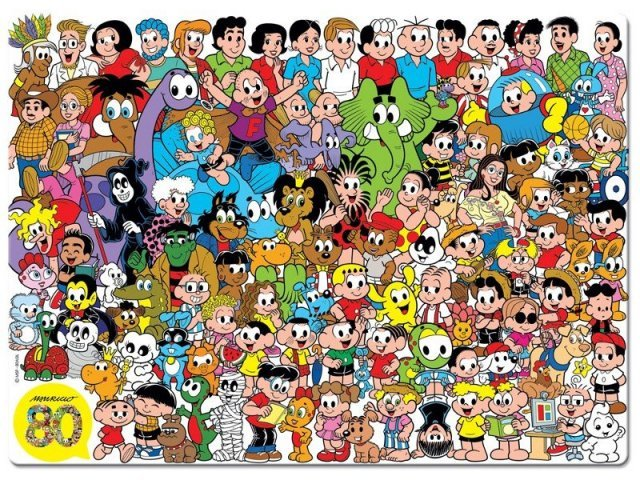
\includegraphics[scale = 0.45]{img/tdm.jpg}
\end{figure}
\end{frame}

% Recapitular primeira apresentação??

\begin{frame}{Rede}
\begin{itemize}
    \item Rede da Turma da Mônica (Clássica e Jovem):
    \begin{itemize}
        \vspace{12pt}
        \item Nós: Personagens;
        \vspace{12pt}
        \item Arestas: Relação de aparecer numa mesma página.
    \end{itemize}
    \vspace{24pt}
\end{itemize}
\end{frame}

\begin{frame}{Rede}
\begin{figure}
    \centering
    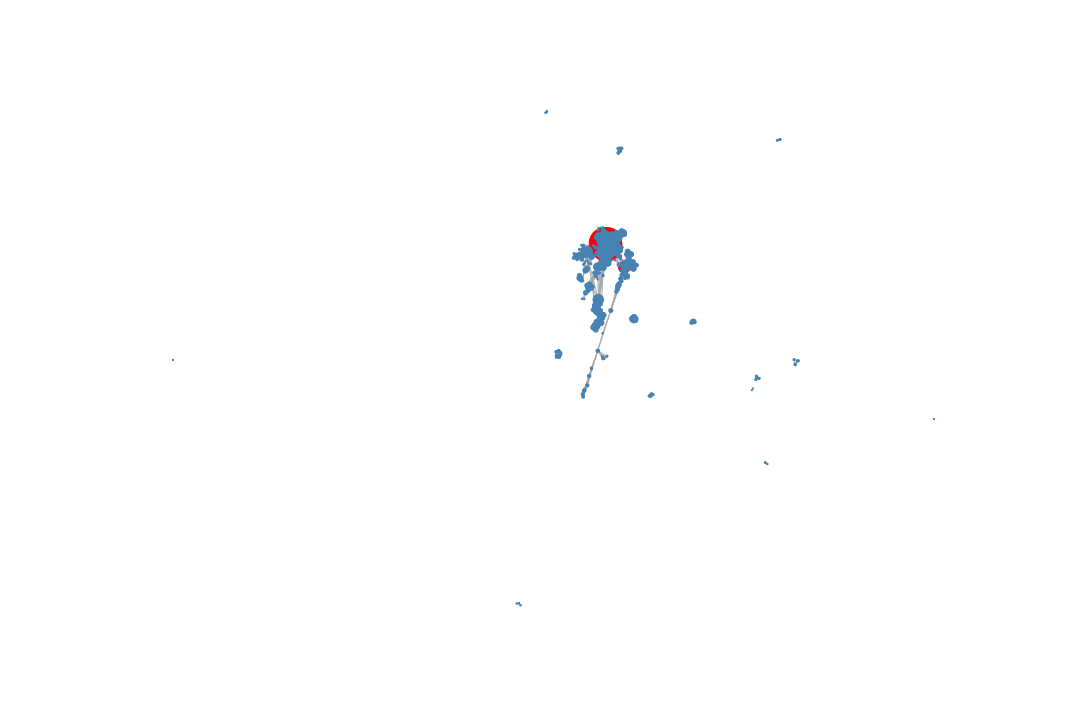
\includegraphics[scale = 0.25]{Second slides set/img/all_comic_books_all_components.png}
    \caption{Rede obtida}
\end{figure}
\end{frame}

\begin{frame}{Rede}
\begin{figure}
    \centering
    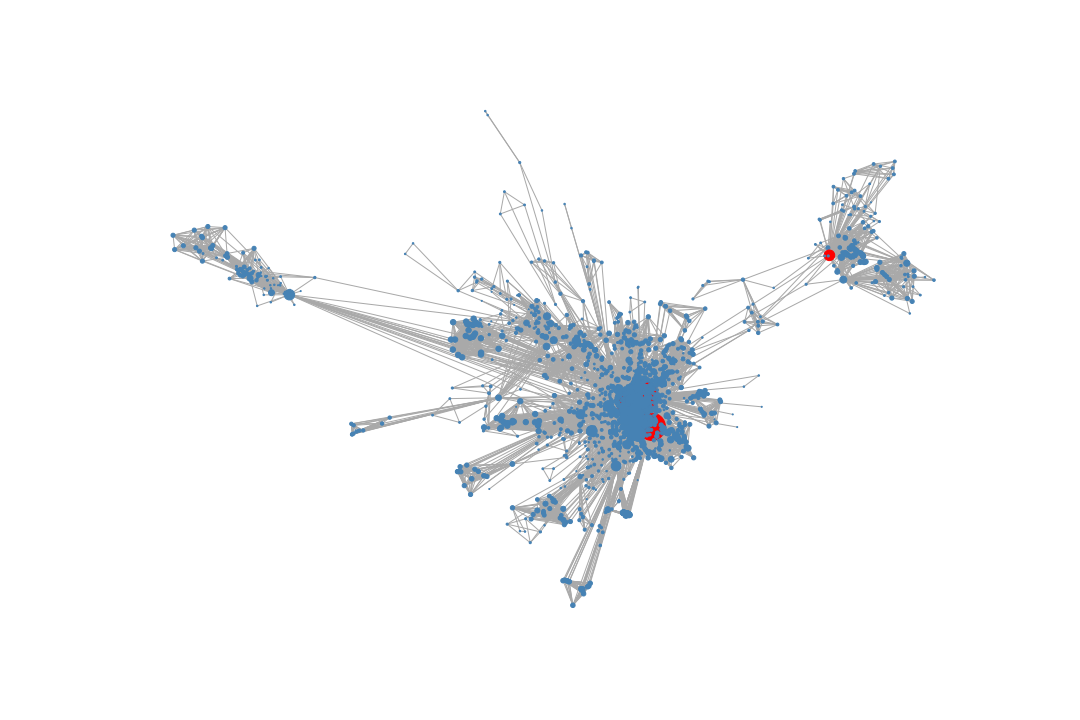
\includegraphics[scale = 0.25]{Second slides set/img/all_comic_books_biggest_component.png}
    \caption{Rede obtida - maior componente conexa}
\end{figure}
\end{frame}

\begin{frame}{Rede - sem figurantes}
\begin{figure}
    \centering
    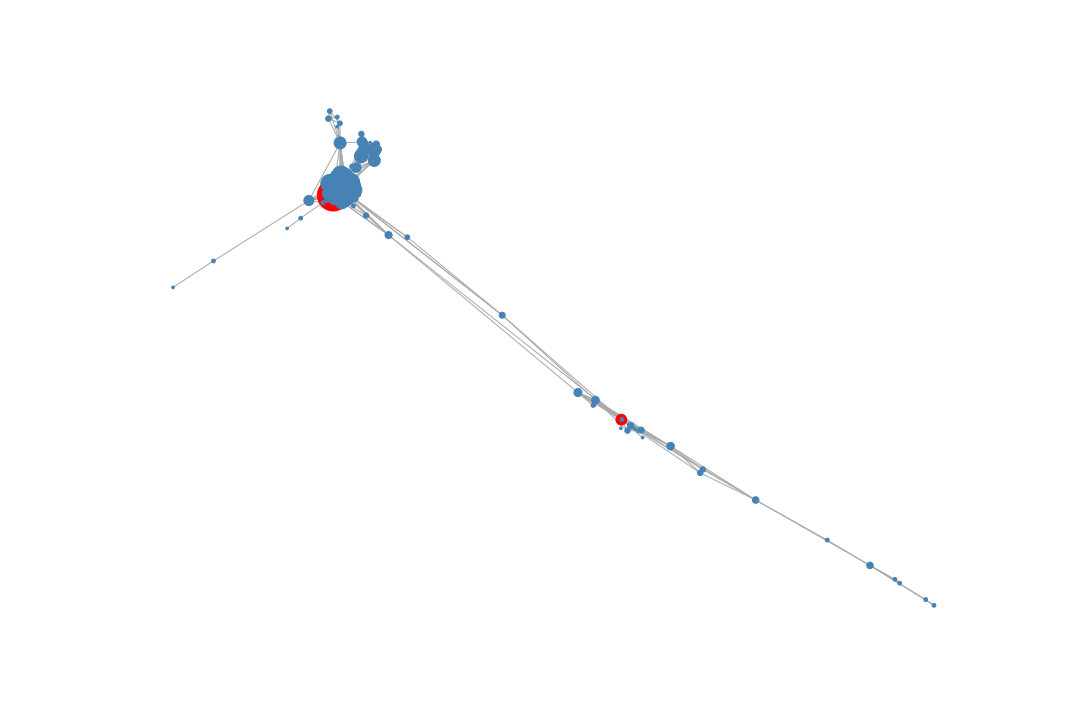
\includegraphics[scale = 0.25]{Second slides set/img/all_comic_books_biggest_component_without_marks.png}
    \caption{Rede obtida sem figurantes}
\end{figure}
\end{frame}

\begin{frame}{Rede}
    Atualizar tabela (ou achar outra forma de mostrar esses dados)
    \begin{table}[]
        \centering
        \begin{tabular}{|l|r|}
            \hline
            Statistic & Value \\ \hline
            Number of nodes & 1845 \\
            Number of edges & 12801 \\
            Average degree & 13.8764 \\
            Density & 0.0075 \\
            Maximum degree & 861 \\
            Degree Standard Deviation & 37.0069 \\
            Diameter & 9 \\
            Average distance & 2.8884 \\
            Number of bridges & 24 \\
            $\frac{\ln{N}}{\ln{<k>}}$ & 2.8592 \\ \hline
        \end{tabular}
        \caption{Dados da Rede}
    \end{table}
\end{frame}

\begin{frame}{Degree Distribuition}
\begin{figure}
    \centering
    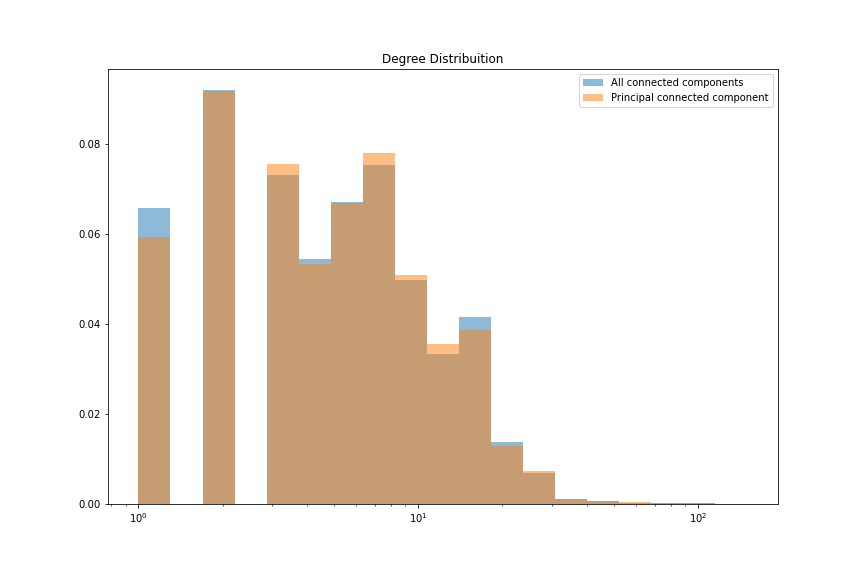
\includegraphics[scale = 0.25]{Second slides set/img/degree_distribuition.png}
    \caption{Distribuição de graus - rede completa}
\end{figure}

Notar que as distribuições são, relativamente, parecidas, exceto que a cauda da distribuição da rede é mais longa
\end{frame}

\begin{frame}{Degree Distribuition}
\begin{figure}
    \centering
    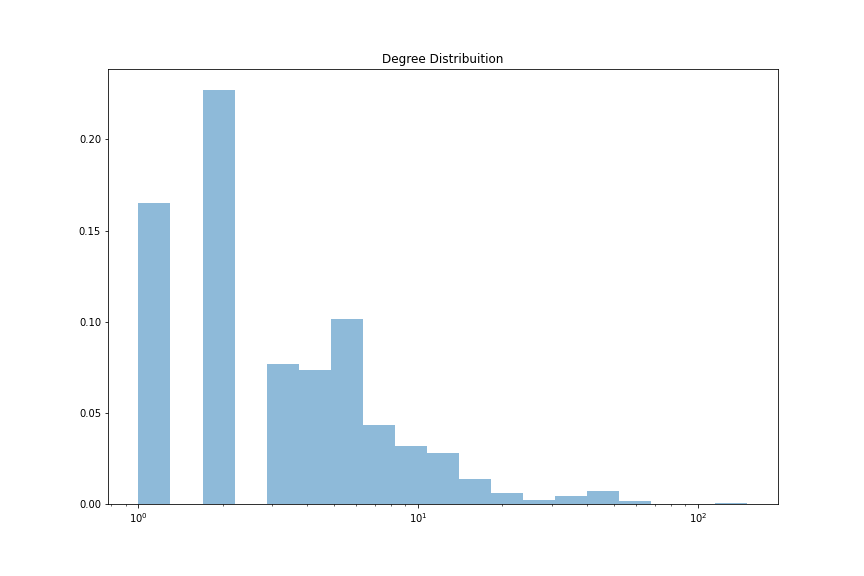
\includegraphics[scale = 0.25]{Second slides set/img/degree_distribuition_without_marks.png}
    \caption{Distribuição de graus - sem figurantes}
\end{figure}

Aqui fica evidente uma separação entre personagens principais, secundários e terciários!
\end{frame}

\begin{frame}{Perguntas}
\begin{itemize}
    \item Qual a distância média entre as personagens?
    \vspace{12pt}
    
    \item Com exceção das personagens principais, quais seriam os maiores HUBs da rede?
    \vspace{12pt}
    
    \item Qual a maior distância entre as personagens?
    \vspace{12pt}
    
    \item Qual o melhor amigo de cada personagem?
    \vspace{12pt}
    
    \item Algoritmos de classificação de comunidades funcionam bem pra separar a rede nas turmas pré-definidas?
\end{itemize}
\end{frame}
    
\begin{frame}{Perguntas}
\begin{itemize}
    \item Qual a distância média entre as personagens? 
    2.9079 na completa e 2.7105 na rede sem figurantes.
    \vspace{12pt}
    
    \item Com exceção das personagens principais, quais seriam os maiores HUBs da rede? 
    Sansão, Denise e Franjinha. Mas se desconsiderarmos os figurantes, Denise dá lugar ao Bidu quando consideramos apenas as conexões (e não seu peso, ou recorrência)!
    \vspace{12pt}
    
    \item Qual a maior distância entre as personagens? 
    9 na rede completa e 8 na rede sem figurantes.
    \vspace{12pt}
    
    \item Qual o melhor amigo de cada personagem?
    \vspace{12pt}
    
    \item Algoritmos de classificação de comunidades funcionam bem pra separar a rede nas turmas pré-definidas?
\end{itemize}
\end{frame}

\begin{frame}{Melhores Amigos}
    Como esperado, os 4 personagens principais são melhores amigos entre si
    
    Seu Souza foi traído pela Dona Luísa. Ele é um cara de família, enquanto ela é bem próxima ao pai do Cascão, o qual é bem próxima a ela também!!
\end{frame}

\begin{frame}{Agradecimentos}
\centering
Obrigado pela atenção!
\end{frame}

\end{document}
